\documentclass[output=paper,
modfonts
]{LSP/langsci}


%%% add all extra packages you need to load to this file 
% \usepackage{todo} %% removed,cna use todonotes instead. % Jason reactivated
% \usepackage{graphicx} % not needed because forest loads tikz, which loads graphicx
\usepackage{tabularx}
\usepackage{amsmath} 
\usepackage{multicol}
\usepackage{lipsum}
\usepackage{longtable}
\usepackage{booktabs}
\usepackage[normalem]{ulem}
%\usepackage{tikz} % not needed because forest loads tikz
\usepackage{phonrule} % for SPE-style phonological rules
\usepackage{pst-all} % loads the main pstricks tools; for arrow diagrams in Hale.tex
%\usepackage{leipzig} % for gloss abbreviations
\usepackage[% for automatic cross-referencing
compress,%
capitalize,% labels are always capitalized in LSP style
noabbrev]% labels are always spelled out in LSP style
{cleveref}

% based on http://tex.stackexchange.com/a/318983/42880 for using gb4e examples with cleveref
\crefname{xnumi}{}{}
\creflabelformat{xnumi}{(#2#1#3)}
\crefrangeformat{xnumi}{(#3#1#4)--(#5#2#6)}
\crefname{xnumii}{}{}
\creflabelformat{xnumii}{(#2#1#3)}
\crefrangeformat{xnumii}{(#3#1#4)--(#5#2#6)}

%\usepackage[notcite,notref]{showkeys} %%removed, not helping CB.
%\usepackage{showidx} %%remove for final compiling - shows index keys at top of page.
 
\usepackage{langsci/styles/langsci-gb4e}  
 \usepackage{pifont}
% % OT tableaux                                                
% \usepackage{pstricks,colortab}  
\usepackage{multirow} % used in OT tableaux
\usepackage{rotating} %needed for angled text%
\usepackage{colortbl} % for cell shading
 
 \usepackage{avm}  
\usepackage[linguistics]{forest} 
\usetikzlibrary{matrix,fit} % for matrix of nodes in Kaisse and Bat-El


\usepackage{hhline}
\newcommand{\cgr}{\cellcolor[gray]{0.8}}
\newcommand{\cn}{\centering}



\newcommand{\reff}[1]{(\ref{#1})}
%\usepackage{newtxtext,newtxmath}


%\usepackage[normalem] {ulem}
\usepackage{qtree}
%\usepackage{natbib}
%\usepackage{tikz}
%\usepackage{gb4e}
\usepackage{phonrule}  
%\bibliographystyle{humannat}



\usepackage{minibox}

%\include{psheader-metr}

\def\bl#1{$_{\textrm{{\footnotesize #1}}}$}

%%%%add all your local new commands to this file

\newcommand{\form}[1]{\mbox{\emph{#1}}}
\newcommand{\uf}[1]{\mbox{/#1/}}

% borrowed from expex and converted from plan tex to latex
\newcommand{\judge}[1]{{\upshape #1\hspace{0.1em}}}
\newcommand{\ljudge}[1]{\makebox[0pt][r]{\judge{#1}}}

\newcommand\tikzmark[1]{\tikz[remember picture, baseline=(#1.base)] \node[anchor=base,inner sep=0pt, outer sep=0pt] (#1) {#1};} % for adding decorations, arrows, lines, etc. to text
\newcommand\tikzmarknamed[2]{\tikz[remember picture, baseline=(#1.base)] \node[anchor=base,inner sep=0pt, outer sep=0pt] (#1) {#2};} % for adding decorations, arrows, lines, etc. to text
\newcommand\tikzmarkfullnamed[2]{\tikz[remember picture, baseline=(#1.base)] \node[anchor=base,inner sep=0pt, outer sep=0pt] (#1) {\vphantom{X}#2};} % for adding decorations, arrows, lines, etc. to text; this one works best for decorations above a line of text because it adds in the heigh of a capital letter and takes two arguments - one for the node name and one for the printed text

\newcommand{\sub}[1]{$_{\text{#1}}$} % for non-math subscripts
\newcommand{\subit}[1]{\sub{\textit{#1}}} % for italics non-math subscripts
\newcommand{\1}{\rlap{$'$}\xspace} % for the prime in X' (the \rlap command allows the prime to be ignored for horizontal spacing in trees, and the \xspace command allows you to use this in normal text without adding \ afterwards). This isn't crucial, but it helps the formatting to look a little better.

% Aissen:
\newcommand\tikzmarkfull[1]{\tikz[remember picture, baseline=(#1.base)] \node[anchor=base,inner sep=0pt, outer sep=0pt] (#1) {\vphantom{X}#1};} % for adding decorations, arrows, lines, etc. to text; this one works best for decorations above a line of text because it adds in the heigh of a capital letter and takes one argument that serves as the name and the printed text
\newcommand{\bridgeover}[2]{% for a line that creates a bridge over text, connecting two nodes
	\begin{tikzpicture}[remember picture,overlay]
	\draw[thick,shorten >=3pt,shorten <=3pt] (#1.north) |- +(0ex,2.5ex) -| (#2.north);
	\end{tikzpicture}
}
\newcommand{\bridgeoverht}[3]{% for a line that creates a bridge over text, connecting two nodes and specifing the height of the bridge
	\begin{tikzpicture}[remember picture,overlay]
	\draw[thick,shorten >=3pt,shorten <=3pt] (#2.north) |- +(0ex,#1) -| (#3.north);
	\end{tikzpicture}
}
\newcommand{\bridgeoverex}{\vspace*{3ex}} % place before an example that has a \bridgeover so that there is enough vertical space for it

% Chung:
\newcommand{\lefttabular}[1]{\begin{tabular}{p{0.5in}}#1\end{tabular}}

% Kaisse:
\newcommand{\mgmorph}[1]{|(#1)| {#1}}
\newcommand{\mgone}[2][$\times$]{\node at (#2.base) [above=2ex] (1#2) {\vphantom{X}#1};}
\newcommand{\mgtwo}[2][$\times$]{\mgone{#2} \node at (#2.base) [above=4.5ex] (2#2) {\vphantom{X}#1};}
\newcommand{\mgthree}[2][$\times$]{\mgtwo{#2} \node at (#2.base) [above=7ex] (3#2) {\vphantom{X}#1};}
\newcommand{\mgftl}[1]{\node at (1#1) [left] {(};}
\newcommand{\mgftr}[1]{\node at (1#1) [right] {)};}
\newcommand{\mgfoot}[2]{\mgftl{#1}\mgftr{#2}}
\newcommand{\mgldelim}[2]{\node at (#2.west) [left,inner sep = 0pt, outer sep = 0pt] {#1};}
\newcommand{\mgrdelim}[2]{\node at (#2.east) [right,inner sep = 0pt, outer sep = 0pt] {#1};}

\newcommand{\squish}{\hspace*{-3pt}}

% Kavitskaya:
\newcommand{\assoc}[2]{\draw (#1.south) -- (#2.north);}
\newcolumntype{L}{>{\raggedright\arraybackslash}X}

% Lepic & Padden:
\newcommand{\fitpic}[1]{\resizebox{\hsize}{!}{\includegraphics{#1}}} % from http://tex.stackexchange.com/a/148965/42880
\newcommand{\signpic}[1]{\includegraphics[width=1.36in]{#1}}
\newcolumntype{C}{>{\centering\arraybackslash}X}

% Spencer:

\newcommand{\textex}[1]{\textit{#1}\xspace}
\newcommand{\lxm}[1]{\textsc{#1}\xspace}

% Thrainsson:

\renewcommand{\textasciitilde}{\char`~} % for use with TTF/OTF fonts (see comments on http://tex.stackexchange.com/a/317/42880)
\newcommand{\tikzarrow}[2]{% for an arrow connecting two nodes
\begin{tikzpicture}[remember picture,overlay]
\draw[thick,shorten >=3pt,shorten <=3pt,->,>=stealth] (#1) -- (#2);
\end{tikzpicture}
}

\newlength{\padding}
\setlength{\padding}{0.5em}
\newcommand{\lesspadding}{\hspace*{-\padding}}
\newcommand{\feat}[1]{\lesspadding#1\lesspadding}

% Hammond

\usepackage[]{graphicx}\usepackage[]{xcolor}
%% maxwidth is the original width if it is less than linewidth
%% otherwise use linewidth (to make sure the graphics do not exceed the margin)
\makeatletter
\def\maxwidth{ %
  \ifdim\Gin@nat@width>\linewidth
    \linewidth
  \else
    \Gin@nat@width
  \fi
}
\makeatother

\definecolor{fgcolor}{rgb}{0.345, 0.345, 0.345}
\newcommand{\hlnum}[1]{\textcolor[rgb]{0.686,0.059,0.569}{#1}}%
\newcommand{\hlstr}[1]{\textcolor[rgb]{0.192,0.494,0.8}{#1}}%
\newcommand{\hlcom}[1]{\textcolor[rgb]{0.678,0.584,0.686}{\textit{#1}}}%
\newcommand{\hlopt}[1]{\textcolor[rgb]{0,0,0}{#1}}%
\newcommand{\hlstd}[1]{\textcolor[rgb]{0.345,0.345,0.345}{#1}}%
\newcommand{\hlkwa}[1]{\textcolor[rgb]{0.161,0.373,0.58}{\textbf{#1}}}%
\newcommand{\hlkwb}[1]{\textcolor[rgb]{0.69,0.353,0.396}{#1}}%
\newcommand{\hlkwc}[1]{\textcolor[rgb]{0.333,0.667,0.333}{#1}}%
\newcommand{\hlkwd}[1]{\textcolor[rgb]{0.737,0.353,0.396}{\textbf{#1}}}%
\let\hlipl\hlkwb

\usepackage{framed}
\makeatletter
\newenvironment{kframe}{%
 \def\at@end@of@kframe{}%
 \ifinner\ifhmode%
  \def\at@end@of@kframe{\end{minipage}}%
  \begin{minipage}{\columnwidth}%
 \fi\fi%
 \def\FrameCommand##1{\hskip\@totalleftmargin \hskip-\fboxsep
 \colorbox{shadecolor}{##1}\hskip-\fboxsep
     % There is no \\@totalrightmargin, so:
     \hskip-\linewidth \hskip-\@totalleftmargin \hskip\columnwidth}%
 \MakeFramed {\advance\hsize-\width
   \@totalleftmargin\z@ \linewidth\hsize
   \@setminipage}}%
 {\par\unskip\endMakeFramed%
 \at@end@of@kframe}
\makeatother

\definecolor{shadecolor}{rgb}{.97, .97, .97}
\definecolor{messagecolor}{rgb}{0, 0, 0}
\definecolor{warningcolor}{rgb}{1, 0, 1}
\definecolor{errorcolor}{rgb}{1, 0, 0}
\newenvironment{knitrout}{}{} % an empty environment to be redefined in TeX

\usepackage{alltt}

%revised version started: 12/17/16

%NEEDS: allbib.bib - already added to the master bibliography file.
%cited references only: bibexport -o mhTMP.bib main1-blx.aux
%PLUS sramh-img*, sramh.tex

%added stuff
\newcommand{\add}[1]{\textcolor{blue}{#1}}
%deleted stuff
\newcommand{\del}[1]{\textcolor{red}{(removed: #1)}}
%uncomment these to turn off colors
\renewcommand{\add}[1]{#1}
\renewcommand{\del}[1]{}

%shortcuts
\newcommand{\w}{\ili{Welsh}}
\newcommand{\e}{\ili{English}}
\newcommand{\io}{Input Optimization}




 \newcommand{\hand}{\ding{43}}
% \newcommand{\rot}[1]{\begin{rotate}{90}#1\end{rotate}} %shortcut for angled text%  
% \newcommand{\rotcon}[1]{\raisebox{-5ex}{\hspace*{1ex}\rot{\hspace*{1ex}#1}}}

%% add all extra packages you need to load to this file 
% \usepackage{todo} %% removed,cna use todonotes instead. % Jason reactivated
% \usepackage{graphicx} % not needed because forest loads tikz, which loads graphicx
\usepackage{tabularx}
\usepackage{amsmath} 
\usepackage{multicol}
\usepackage{lipsum}
\usepackage{longtable}
\usepackage{booktabs}
\usepackage[normalem]{ulem}
%\usepackage{tikz} % not needed because forest loads tikz
\usepackage{phonrule} % for SPE-style phonological rules
\usepackage{pst-all} % loads the main pstricks tools; for arrow diagrams in Hale.tex
%\usepackage{leipzig} % for gloss abbreviations
\usepackage[% for automatic cross-referencing
compress,%
capitalize,% labels are always capitalized in LSP style
noabbrev]% labels are always spelled out in LSP style
{cleveref}

% based on http://tex.stackexchange.com/a/318983/42880 for using gb4e examples with cleveref
\crefname{xnumi}{}{}
\creflabelformat{xnumi}{(#2#1#3)}
\crefrangeformat{xnumi}{(#3#1#4)--(#5#2#6)}
\crefname{xnumii}{}{}
\creflabelformat{xnumii}{(#2#1#3)}
\crefrangeformat{xnumii}{(#3#1#4)--(#5#2#6)}

%\usepackage[notcite,notref]{showkeys} %%removed, not helping CB.
%\usepackage{showidx} %%remove for final compiling - shows index keys at top of page.
 
\usepackage{langsci/styles/langsci-gb4e}  
 \usepackage{pifont}
% % OT tableaux                                                
% \usepackage{pstricks,colortab}  
\usepackage{multirow} % used in OT tableaux
\usepackage{rotating} %needed for angled text%
\usepackage{colortbl} % for cell shading
 
 \usepackage{avm}  
\usepackage[linguistics]{forest} 
\usetikzlibrary{matrix,fit} % for matrix of nodes in Kaisse and Bat-El


\usepackage{hhline}
\newcommand{\cgr}{\cellcolor[gray]{0.8}}
\newcommand{\cn}{\centering}



\newcommand{\reff}[1]{(\ref{#1})}
%\usepackage{newtxtext,newtxmath}


%\usepackage[normalem] {ulem}
\usepackage{qtree}
%\usepackage{natbib}
%\usepackage{tikz}
%\usepackage{gb4e}
\usepackage{phonrule}  
%\bibliographystyle{humannat}



\usepackage{minibox}

%\include{psheader-metr}

\def\bl#1{$_{\textrm{{\footnotesize #1}}}$}
\usepackage{arydshln}
\usepackage{rotating}

%%add all your local new commands to this file

\newcommand{\form}[1]{\mbox{\emph{#1}}}
\newcommand{\uf}[1]{\mbox{/#1/}}

% borrowed from expex and converted from plan tex to latex
\newcommand{\judge}[1]{{\upshape #1\hspace{0.1em}}}
\newcommand{\ljudge}[1]{\makebox[0pt][r]{\judge{#1}}}

\newcommand\tikzmark[1]{\tikz[remember picture, baseline=(#1.base)] \node[anchor=base,inner sep=0pt, outer sep=0pt] (#1) {#1};} % for adding decorations, arrows, lines, etc. to text
\newcommand\tikzmarknamed[2]{\tikz[remember picture, baseline=(#1.base)] \node[anchor=base,inner sep=0pt, outer sep=0pt] (#1) {#2};} % for adding decorations, arrows, lines, etc. to text
\newcommand\tikzmarkfullnamed[2]{\tikz[remember picture, baseline=(#1.base)] \node[anchor=base,inner sep=0pt, outer sep=0pt] (#1) {\vphantom{X}#2};} % for adding decorations, arrows, lines, etc. to text; this one works best for decorations above a line of text because it adds in the heigh of a capital letter and takes two arguments - one for the node name and one for the printed text

\newcommand{\sub}[1]{$_{\text{#1}}$} % for non-math subscripts
\newcommand{\subit}[1]{\sub{\textit{#1}}} % for italics non-math subscripts
\newcommand{\1}{\rlap{$'$}\xspace} % for the prime in X' (the \rlap command allows the prime to be ignored for horizontal spacing in trees, and the \xspace command allows you to use this in normal text without adding \ afterwards). This isn't crucial, but it helps the formatting to look a little better.

% Aissen:
\newcommand\tikzmarkfull[1]{\tikz[remember picture, baseline=(#1.base)] \node[anchor=base,inner sep=0pt, outer sep=0pt] (#1) {\vphantom{X}#1};} % for adding decorations, arrows, lines, etc. to text; this one works best for decorations above a line of text because it adds in the heigh of a capital letter and takes one argument that serves as the name and the printed text
\newcommand{\bridgeover}[2]{% for a line that creates a bridge over text, connecting two nodes
	\begin{tikzpicture}[remember picture,overlay]
	\draw[thick,shorten >=3pt,shorten <=3pt] (#1.north) |- +(0ex,2.5ex) -| (#2.north);
	\end{tikzpicture}
}
\newcommand{\bridgeoverht}[3]{% for a line that creates a bridge over text, connecting two nodes and specifing the height of the bridge
	\begin{tikzpicture}[remember picture,overlay]
	\draw[thick,shorten >=3pt,shorten <=3pt] (#2.north) |- +(0ex,#1) -| (#3.north);
	\end{tikzpicture}
}
\newcommand{\bridgeoverex}{\vspace*{3ex}} % place before an example that has a \bridgeover so that there is enough vertical space for it

% Chung:
\newcommand{\lefttabular}[1]{\begin{tabular}{p{0.5in}}#1\end{tabular}}

% Kaisse:
\newcommand{\mgmorph}[1]{|(#1)| {#1}}
\newcommand{\mgone}[2][$\times$]{\node at (#2.base) [above=2ex] (1#2) {\vphantom{X}#1};}
\newcommand{\mgtwo}[2][$\times$]{\mgone{#2} \node at (#2.base) [above=4.5ex] (2#2) {\vphantom{X}#1};}
\newcommand{\mgthree}[2][$\times$]{\mgtwo{#2} \node at (#2.base) [above=7ex] (3#2) {\vphantom{X}#1};}
\newcommand{\mgftl}[1]{\node at (1#1) [left] {(};}
\newcommand{\mgftr}[1]{\node at (1#1) [right] {)};}
\newcommand{\mgfoot}[2]{\mgftl{#1}\mgftr{#2}}
\newcommand{\mgldelim}[2]{\node at (#2.west) [left,inner sep = 0pt, outer sep = 0pt] {#1};}
\newcommand{\mgrdelim}[2]{\node at (#2.east) [right,inner sep = 0pt, outer sep = 0pt] {#1};}

\newcommand{\squish}{\hspace*{-3pt}}

% Kavitskaya:
\newcommand{\assoc}[2]{\draw (#1.south) -- (#2.north);}
\newcolumntype{L}{>{\raggedright\arraybackslash}X}

% Lepic & Padden:
\newcommand{\fitpic}[1]{\resizebox{\hsize}{!}{\includegraphics{#1}}} % from http://tex.stackexchange.com/a/148965/42880
\newcommand{\signpic}[1]{\includegraphics[width=1.36in]{#1}}
\newcolumntype{C}{>{\centering\arraybackslash}X}

% Spencer:

\newcommand{\textex}[1]{\textit{#1}\xspace}
\newcommand{\lxm}[1]{\textsc{#1}\xspace}

% Thrainsson:

\renewcommand{\textasciitilde}{\char`~} % for use with TTF/OTF fonts (see comments on http://tex.stackexchange.com/a/317/42880)
\newcommand{\tikzarrow}[2]{% for an arrow connecting two nodes
\begin{tikzpicture}[remember picture,overlay]
\draw[thick,shorten >=3pt,shorten <=3pt,->,>=stealth] (#1) -- (#2);
\end{tikzpicture}
}

\newlength{\padding}
\setlength{\padding}{0.5em}
\newcommand{\lesspadding}{\hspace*{-\padding}}
\newcommand{\feat}[1]{\lesspadding#1\lesspadding}

% Hammond

\usepackage[]{graphicx}\usepackage[]{xcolor}
%% maxwidth is the original width if it is less than linewidth
%% otherwise use linewidth (to make sure the graphics do not exceed the margin)
\makeatletter
\def\maxwidth{ %
  \ifdim\Gin@nat@width>\linewidth
    \linewidth
  \else
    \Gin@nat@width
  \fi
}
\makeatother

\definecolor{fgcolor}{rgb}{0.345, 0.345, 0.345}
\newcommand{\hlnum}[1]{\textcolor[rgb]{0.686,0.059,0.569}{#1}}%
\newcommand{\hlstr}[1]{\textcolor[rgb]{0.192,0.494,0.8}{#1}}%
\newcommand{\hlcom}[1]{\textcolor[rgb]{0.678,0.584,0.686}{\textit{#1}}}%
\newcommand{\hlopt}[1]{\textcolor[rgb]{0,0,0}{#1}}%
\newcommand{\hlstd}[1]{\textcolor[rgb]{0.345,0.345,0.345}{#1}}%
\newcommand{\hlkwa}[1]{\textcolor[rgb]{0.161,0.373,0.58}{\textbf{#1}}}%
\newcommand{\hlkwb}[1]{\textcolor[rgb]{0.69,0.353,0.396}{#1}}%
\newcommand{\hlkwc}[1]{\textcolor[rgb]{0.333,0.667,0.333}{#1}}%
\newcommand{\hlkwd}[1]{\textcolor[rgb]{0.737,0.353,0.396}{\textbf{#1}}}%
\let\hlipl\hlkwb

\usepackage{framed}
\makeatletter
\newenvironment{kframe}{%
 \def\at@end@of@kframe{}%
 \ifinner\ifhmode%
  \def\at@end@of@kframe{\end{minipage}}%
  \begin{minipage}{\columnwidth}%
 \fi\fi%
 \def\FrameCommand##1{\hskip\@totalleftmargin \hskip-\fboxsep
 \colorbox{shadecolor}{##1}\hskip-\fboxsep
     % There is no \\@totalrightmargin, so:
     \hskip-\linewidth \hskip-\@totalleftmargin \hskip\columnwidth}%
 \MakeFramed {\advance\hsize-\width
   \@totalleftmargin\z@ \linewidth\hsize
   \@setminipage}}%
 {\par\unskip\endMakeFramed%
 \at@end@of@kframe}
\makeatother

\definecolor{shadecolor}{rgb}{.97, .97, .97}
\definecolor{messagecolor}{rgb}{0, 0, 0}
\definecolor{warningcolor}{rgb}{1, 0, 1}
\definecolor{errorcolor}{rgb}{1, 0, 0}
\newenvironment{knitrout}{}{} % an empty environment to be redefined in TeX

\usepackage{alltt}

%revised version started: 12/17/16

%NEEDS: allbib.bib - already added to the master bibliography file.
%cited references only: bibexport -o mhTMP.bib main1-blx.aux
%PLUS sramh-img*, sramh.tex

%added stuff
\newcommand{\add}[1]{\textcolor{blue}{#1}}
%deleted stuff
\newcommand{\del}[1]{\textcolor{red}{(removed: #1)}}
%uncomment these to turn off colors
\renewcommand{\add}[1]{#1}
\renewcommand{\del}[1]{}

%shortcuts
\newcommand{\w}{\ili{Welsh}}
\newcommand{\e}{\ili{English}}
\newcommand{\io}{Input Optimization}




 \newcommand{\hand}{\ding{43}}
% \newcommand{\rot}[1]{\begin{rotate}{90}#1\end{rotate}} %shortcut for angled text%  
% \newcommand{\rotcon}[1]{\raisebox{-5ex}{\hspace*{1ex}\rot{\hspace*{1ex}#1}}}

%% add all extra packages you need to load to this file 
% \usepackage{todo} %% removed,cna use todonotes instead. % Jason reactivated
% \usepackage{graphicx} % not needed because forest loads tikz, which loads graphicx
\usepackage{tabularx}
\usepackage{amsmath} 
\usepackage{multicol}
\usepackage{lipsum}
\usepackage{longtable}
\usepackage{booktabs}
\usepackage[normalem]{ulem}
%\usepackage{tikz} % not needed because forest loads tikz
\usepackage{phonrule} % for SPE-style phonological rules
\usepackage{pst-all} % loads the main pstricks tools; for arrow diagrams in Hale.tex
%\usepackage{leipzig} % for gloss abbreviations
\usepackage[% for automatic cross-referencing
compress,%
capitalize,% labels are always capitalized in LSP style
noabbrev]% labels are always spelled out in LSP style
{cleveref}

% based on http://tex.stackexchange.com/a/318983/42880 for using gb4e examples with cleveref
\crefname{xnumi}{}{}
\creflabelformat{xnumi}{(#2#1#3)}
\crefrangeformat{xnumi}{(#3#1#4)--(#5#2#6)}
\crefname{xnumii}{}{}
\creflabelformat{xnumii}{(#2#1#3)}
\crefrangeformat{xnumii}{(#3#1#4)--(#5#2#6)}

%\usepackage[notcite,notref]{showkeys} %%removed, not helping CB.
%\usepackage{showidx} %%remove for final compiling - shows index keys at top of page.
 
\usepackage{langsci/styles/langsci-gb4e}  
 \usepackage{pifont}
% % OT tableaux                                                
% \usepackage{pstricks,colortab}  
\usepackage{multirow} % used in OT tableaux
\usepackage{rotating} %needed for angled text%
\usepackage{colortbl} % for cell shading
 
 \usepackage{avm}  
\usepackage[linguistics]{forest} 
\usetikzlibrary{matrix,fit} % for matrix of nodes in Kaisse and Bat-El


\usepackage{hhline}
\newcommand{\cgr}{\cellcolor[gray]{0.8}}
\newcommand{\cn}{\centering}



\newcommand{\reff}[1]{(\ref{#1})}
%\usepackage{newtxtext,newtxmath}


%\usepackage[normalem] {ulem}
\usepackage{qtree}
%\usepackage{natbib}
%\usepackage{tikz}
%\usepackage{gb4e}
\usepackage{phonrule}  
%\bibliographystyle{humannat}



\usepackage{minibox}

%\include{psheader-metr}

\def\bl#1{$_{\textrm{{\footnotesize #1}}}$}
\usepackage{arydshln}
\usepackage{rotating}

%%add all your local new commands to this file

\newcommand{\form}[1]{\mbox{\emph{#1}}}
\newcommand{\uf}[1]{\mbox{/#1/}}

% borrowed from expex and converted from plan tex to latex
\newcommand{\judge}[1]{{\upshape #1\hspace{0.1em}}}
\newcommand{\ljudge}[1]{\makebox[0pt][r]{\judge{#1}}}

\newcommand\tikzmark[1]{\tikz[remember picture, baseline=(#1.base)] \node[anchor=base,inner sep=0pt, outer sep=0pt] (#1) {#1};} % for adding decorations, arrows, lines, etc. to text
\newcommand\tikzmarknamed[2]{\tikz[remember picture, baseline=(#1.base)] \node[anchor=base,inner sep=0pt, outer sep=0pt] (#1) {#2};} % for adding decorations, arrows, lines, etc. to text
\newcommand\tikzmarkfullnamed[2]{\tikz[remember picture, baseline=(#1.base)] \node[anchor=base,inner sep=0pt, outer sep=0pt] (#1) {\vphantom{X}#2};} % for adding decorations, arrows, lines, etc. to text; this one works best for decorations above a line of text because it adds in the heigh of a capital letter and takes two arguments - one for the node name and one for the printed text

\newcommand{\sub}[1]{$_{\text{#1}}$} % for non-math subscripts
\newcommand{\subit}[1]{\sub{\textit{#1}}} % for italics non-math subscripts
\newcommand{\1}{\rlap{$'$}\xspace} % for the prime in X' (the \rlap command allows the prime to be ignored for horizontal spacing in trees, and the \xspace command allows you to use this in normal text without adding \ afterwards). This isn't crucial, but it helps the formatting to look a little better.

% Aissen:
\newcommand\tikzmarkfull[1]{\tikz[remember picture, baseline=(#1.base)] \node[anchor=base,inner sep=0pt, outer sep=0pt] (#1) {\vphantom{X}#1};} % for adding decorations, arrows, lines, etc. to text; this one works best for decorations above a line of text because it adds in the heigh of a capital letter and takes one argument that serves as the name and the printed text
\newcommand{\bridgeover}[2]{% for a line that creates a bridge over text, connecting two nodes
	\begin{tikzpicture}[remember picture,overlay]
	\draw[thick,shorten >=3pt,shorten <=3pt] (#1.north) |- +(0ex,2.5ex) -| (#2.north);
	\end{tikzpicture}
}
\newcommand{\bridgeoverht}[3]{% for a line that creates a bridge over text, connecting two nodes and specifing the height of the bridge
	\begin{tikzpicture}[remember picture,overlay]
	\draw[thick,shorten >=3pt,shorten <=3pt] (#2.north) |- +(0ex,#1) -| (#3.north);
	\end{tikzpicture}
}
\newcommand{\bridgeoverex}{\vspace*{3ex}} % place before an example that has a \bridgeover so that there is enough vertical space for it

% Chung:
\newcommand{\lefttabular}[1]{\begin{tabular}{p{0.5in}}#1\end{tabular}}

% Kaisse:
\newcommand{\mgmorph}[1]{|(#1)| {#1}}
\newcommand{\mgone}[2][$\times$]{\node at (#2.base) [above=2ex] (1#2) {\vphantom{X}#1};}
\newcommand{\mgtwo}[2][$\times$]{\mgone{#2} \node at (#2.base) [above=4.5ex] (2#2) {\vphantom{X}#1};}
\newcommand{\mgthree}[2][$\times$]{\mgtwo{#2} \node at (#2.base) [above=7ex] (3#2) {\vphantom{X}#1};}
\newcommand{\mgftl}[1]{\node at (1#1) [left] {(};}
\newcommand{\mgftr}[1]{\node at (1#1) [right] {)};}
\newcommand{\mgfoot}[2]{\mgftl{#1}\mgftr{#2}}
\newcommand{\mgldelim}[2]{\node at (#2.west) [left,inner sep = 0pt, outer sep = 0pt] {#1};}
\newcommand{\mgrdelim}[2]{\node at (#2.east) [right,inner sep = 0pt, outer sep = 0pt] {#1};}

\newcommand{\squish}{\hspace*{-3pt}}

% Kavitskaya:
\newcommand{\assoc}[2]{\draw (#1.south) -- (#2.north);}
\newcolumntype{L}{>{\raggedright\arraybackslash}X}

% Lepic & Padden:
\newcommand{\fitpic}[1]{\resizebox{\hsize}{!}{\includegraphics{#1}}} % from http://tex.stackexchange.com/a/148965/42880
\newcommand{\signpic}[1]{\includegraphics[width=1.36in]{#1}}
\newcolumntype{C}{>{\centering\arraybackslash}X}

% Spencer:

\newcommand{\textex}[1]{\textit{#1}\xspace}
\newcommand{\lxm}[1]{\textsc{#1}\xspace}

% Thrainsson:

\renewcommand{\textasciitilde}{\char`~} % for use with TTF/OTF fonts (see comments on http://tex.stackexchange.com/a/317/42880)
\newcommand{\tikzarrow}[2]{% for an arrow connecting two nodes
\begin{tikzpicture}[remember picture,overlay]
\draw[thick,shorten >=3pt,shorten <=3pt,->,>=stealth] (#1) -- (#2);
\end{tikzpicture}
}

\newlength{\padding}
\setlength{\padding}{0.5em}
\newcommand{\lesspadding}{\hspace*{-\padding}}
\newcommand{\feat}[1]{\lesspadding#1\lesspadding}

% Hammond

\usepackage[]{graphicx}\usepackage[]{xcolor}
%% maxwidth is the original width if it is less than linewidth
%% otherwise use linewidth (to make sure the graphics do not exceed the margin)
\makeatletter
\def\maxwidth{ %
  \ifdim\Gin@nat@width>\linewidth
    \linewidth
  \else
    \Gin@nat@width
  \fi
}
\makeatother

\definecolor{fgcolor}{rgb}{0.345, 0.345, 0.345}
\newcommand{\hlnum}[1]{\textcolor[rgb]{0.686,0.059,0.569}{#1}}%
\newcommand{\hlstr}[1]{\textcolor[rgb]{0.192,0.494,0.8}{#1}}%
\newcommand{\hlcom}[1]{\textcolor[rgb]{0.678,0.584,0.686}{\textit{#1}}}%
\newcommand{\hlopt}[1]{\textcolor[rgb]{0,0,0}{#1}}%
\newcommand{\hlstd}[1]{\textcolor[rgb]{0.345,0.345,0.345}{#1}}%
\newcommand{\hlkwa}[1]{\textcolor[rgb]{0.161,0.373,0.58}{\textbf{#1}}}%
\newcommand{\hlkwb}[1]{\textcolor[rgb]{0.69,0.353,0.396}{#1}}%
\newcommand{\hlkwc}[1]{\textcolor[rgb]{0.333,0.667,0.333}{#1}}%
\newcommand{\hlkwd}[1]{\textcolor[rgb]{0.737,0.353,0.396}{\textbf{#1}}}%
\let\hlipl\hlkwb

\usepackage{framed}
\makeatletter
\newenvironment{kframe}{%
 \def\at@end@of@kframe{}%
 \ifinner\ifhmode%
  \def\at@end@of@kframe{\end{minipage}}%
  \begin{minipage}{\columnwidth}%
 \fi\fi%
 \def\FrameCommand##1{\hskip\@totalleftmargin \hskip-\fboxsep
 \colorbox{shadecolor}{##1}\hskip-\fboxsep
     % There is no \\@totalrightmargin, so:
     \hskip-\linewidth \hskip-\@totalleftmargin \hskip\columnwidth}%
 \MakeFramed {\advance\hsize-\width
   \@totalleftmargin\z@ \linewidth\hsize
   \@setminipage}}%
 {\par\unskip\endMakeFramed%
 \at@end@of@kframe}
\makeatother

\definecolor{shadecolor}{rgb}{.97, .97, .97}
\definecolor{messagecolor}{rgb}{0, 0, 0}
\definecolor{warningcolor}{rgb}{1, 0, 1}
\definecolor{errorcolor}{rgb}{1, 0, 0}
\newenvironment{knitrout}{}{} % an empty environment to be redefined in TeX

\usepackage{alltt}

%revised version started: 12/17/16

%NEEDS: allbib.bib - already added to the master bibliography file.
%cited references only: bibexport -o mhTMP.bib main1-blx.aux
%PLUS sramh-img*, sramh.tex

%added stuff
\newcommand{\add}[1]{\textcolor{blue}{#1}}
%deleted stuff
\newcommand{\del}[1]{\textcolor{red}{(removed: #1)}}
%uncomment these to turn off colors
\renewcommand{\add}[1]{#1}
\renewcommand{\del}[1]{}

%shortcuts
\newcommand{\w}{\ili{Welsh}}
\newcommand{\e}{\ili{English}}
\newcommand{\io}{Input Optimization}




 \newcommand{\hand}{\ding{43}}
% \newcommand{\rot}[1]{\begin{rotate}{90}#1\end{rotate}} %shortcut for angled text%  
% \newcommand{\rotcon}[1]{\raisebox{-5ex}{\hspace*{1ex}\rot{\hspace*{1ex}#1}}}

%\input{localpackages.tex}
\usepackage{arydshln}
\usepackage{rotating}

%\input{localcommands.tex}
\newcommand{\tworow}[1]{\multirow{2}{*}{#1}}


\newcommand{\tworow}[1]{\multirow{2}{*}{#1}}


\newcommand{\tworow}[1]{\multirow{2}{*}{#1}}



\graphicspath{{./figures/goldstein/}}

\title{Temporal patterning in speech and birdsong}
\author{Louis Goldstein\affiliation{Department of Linguistics, University of Southern California}}

% \chapterDOI{} %will be filled in at production
% \epigram{}

\abstract{
Speech and birdsong are complex motor behaviors in which patterning over time is itself informational. This is obvious in the case of speech, but in birdsong, too, the sequencing (and possibly timing) of syllables determines in part the well-formedness of the song. Despite gross differences in function, in the physical substrate (method of sound production), in brain structure, and in the scale of the animals, recent work has revealed a surprising degree of similarity in their solutions to the problem of controlling temporal patterning.  There are differences, too, of course, and when we find them, it deepens our understanding about the (unique) structure of speech. Because Steve has had a lasting interest in birds and birdsong \citep{Anderson2006}, this seemed to be an appropriate context to review these similarities. Two of them will be the focus of discussion here: decomposition of the behavior into a \textit{sequence of discrete motor units} and the role of an \textit{internal clock system}, partly independent of the units themselves.

}

\begin{document}
\maketitle

\section{Discrete decomposition}
%\label{sec:discrete}

One of the foundational motivations for Articulatory Phonology (\citealt{BG92, BG95}) is to address the apparent incompatibility between the discrete phonetic and phonological structure of speech, on the one hand,  and the observation that the vocal tract articulators move in a continuous fashion, producing continuous modulation of the acoustics, on the other.  AP hypothesizes that it is possible to model the continuous motion of the articulators as arising from discrete, context-independent dynamical control systems, called \textit{gestures}, that govern the formation of phonologically-relevant constrictions within the vocal tract (for example bringing the tongue tip to the palate, with a particular degree of constriction). The control parameters of these dynamical systems (\textit{target}, e.g., the phonologically-specified degree of constriction,  and \textit{stiffness}, the time constant that determines the amount of time required for the system to settle at its target value) remain fixed during the duration of the constriction action (roughly a consonant or a vowel), even though the articulators are moving. The decomposition of speech into a pattern of gesture activations over time (or \textit{gestural score}), is an abstract analysis (as Steve argued in his earliest work \citep{anderson74} must be the case for a phonetic representation), and can only be discovered by use of  explicit dynamical and acoustical models.  We cannot observe it directly. Recently,  Nam et al  \citeyearpar{Nam2012} showed that with the use of the TaDA gestural production model, it is possible to parse an acoustic signal into the maximum likelihood gestural score that could have produced it.

A similar strategy is employed by \citet{Amador2013}, to decompose zebra finch song into discrete gestures. The authors first developed a dynamical model of sound production in the syrinx, the sound production organ in songbirds. The syrinx is a vibratory system located at the base of the trachea. The trachea divides into two tubes at that point, each of which hosts a pair of vibrating membranes called labia. The two pairs of labia can vibrate together or separately, or can be sequenced \citep{RiedeGoller}.  The model developed in \citet{Amador2013} (for a single pair of labia) allowed them to generate sound from two dynamical control parameters: the average tension in the labia, and tracheal pressure. Then, using a table-lookup scheme, they were able to estimate the time functions of these two parameters from audio recordings of the sound. This representation was then validated by generating audio from those time functions and playing those sounds to zebra finches. Neural responses from the synthetic song were highly similar (nearly identical) to the responses obtained by playing the original song (BOS, Bird's Own Song). Next, they showed that the derived time functions are essentially discrete: they exhibit sequences of intervals of time during which the values of the control parameters remain essentially fixed (just as with speech gestures), and refer to these intervals as elemental gestures of the song. The key similarity to speech gestures is that the continuous song can be decomposed into discrete intervals of time, longer by an order of magnitude than the periodicity of the song, during which the dynamical parameters are essentially fixed. 

There are also some salient differences between speech gestures and zebra finch song gestures. Most superficial is that the control parameters for the zebra finch gestures are different from those of speech gestures that control the constrictions of the suprlaryngeal structures (as expected, because forming constrictions is not generally thought to be part of the bird's song behavior), but they are similar to those control parameters involved in controlling tone and intonation in speech \citep{McGowanSaltz}. 
A somewhat deeper difference is that the zebra finch gestures (as analyzed in \citealt{Amador2013}) are strictly sequential, while speech gestures exhibit various types of overlap in time. At first blush, this makes sense, as the mechanism of sound production in birds is generally thought to be limited to a single device, the syrinx, while the distinct vocal organs of the human vocal tract can each make their own contribution to the filtering action of sound generated at the larynx. There are, however, as noted above, two sets of labia comprising the syrinx \citep{Trevas2007}, and some avian species employ primarily one set, while others (like zebra finches) use both sets, simultaneously or sequentially.   Trevisian et al. \citeyearpar{Trevas2007} have shown how such symmetry-breaking (different functioning of the two sides at the same time) arises in the species that employ either one side only or both sides, but not symmetrically. So there is the possibility that distinct patterns of gesture overlap may yet be uncovered.

%% come back to this
Another obvious potential difference is compositionality. A small set of discrete speech gestures are employed in different combinations to create the set of segments and syllables in a language. It is unknown whether gestures in birdsong are compositional in this sense. Zebra finch songs (on which a large bulk of the research on song birds has been done) have been described as having a hierarchical structure. Syllables are the most immediately identifiable units, as they consist of the vocalization intervals produced by the bird that are bounded by (silent) inspirations. The total number of distinct syllables in a given bird's inventory is relatively small, on the order of 20 or so. As described in \citet{YuMargoliash96},  syllables can be composed of distinct notes, and in turn, sequences of syllables form \textit{motifs}, that can be repeated as part of a song. It is unclear to what extent the elemental gestures identified in \citet{Amador2013} can form parts of more than one syllable in an individual's inventory.  Yu and Margoliash \citeyearpar{YuMargoliash96} do report instances of distinct syllables in a bird's inventory that begin with the same note (and end with different notes). To the extent that those shared notes are produced with the same gestures, this would be evidence for some limited compositionality.

\section{Clocks}
%\label{sec:clocks}

\subsection{Clocks in speech?}
A lively debate in the 1980's sparked by the work of Carol Fowler \citep{Fowler80} considered whether speech units had their own intrinsic timing as dynamical systems (as argued by Fowler), or whether the timing is imposed externally by some kind of central clock. Gestures in Articulatory Phonology are units with intrinsic timing; the time required for a gesture to reach its goal state is determined by its dynamical stiffness parameter. But what of the time between gestures? For a sequence of two gestures, $x{_1}$ and $x{_2}$, we can ask how the system controls when to trigger $x{_2}$ with respect to $x{_1}$. A natural answer to this is that $x{_2}$ is triggered when some reference state value of $x{_1}$ is achieved $\{x{_1}, \dot{x{_1}}\}$. Sequencing in motor systems is often modeled by a mechanism of ``competitive selection'' of the sequenced items \citep{Bullock2002,Grossberg78}, where feedback from the completion of element $x{_1}$ (achievement of its target state) allows it to be deactivated and element $x{_2}$ to be selected and triggered.  In the case of speech, this feedback could be kinesthetic, orosensory and/or acoustic. However, there is an argument that this cannot be the complete story for speech. Consider the gestural score for the word ``spot'' in the left panel of Figure~\ref{fig:spot}. The boxes represent intervals in which the the supralaryngeal gestures would be active, in some token of this word. The onset of the lip closure for /p/ initiates at a moment when the tongue tip fricative gesture (for /s/) is at a particular state (close to its target and not moving much), as marked by the vertical line in the figure. A possible mechanism for sequencing the these gestures would be to learn that in producing the word ``spot,'' the lip closure gesture ``waits'' until the system has feedback that the tongue tip is near the alveolar ridge and is moving with little velocity, and at that point it is triggered.   But now consider the phrase ``toss spot'' shown on the right side of Figure \ref{fig:spot}. Here, the state that the lip closure is looking for, in order to trigger, occurs too early, because the tongue tip is already in position for /s/. And there is a interval of time (shaded in white) during which the state of the tongue tip does not change much, so there is no information in its state that can inform when the /p/ should be triggered. Nonetheless, its timing must show some regularity, as the [s] in ``toss spot'' systematically differs in duration from, for example ``pa spot.'' Figure \ref{fig:had-tied} shows the kinematics of the tongue tip in a sequence of identical supralaryngeal gestures (``had tied'').  It is clear that there is indeed a considerable stretch (70 ms or so) marked with a yellow box  where its state does not change, and so information about when to trigger a next gesture is lacking. 

This case appears to argue that a simple state-based chain triggering will not work for speech, in the general case, and relative timing must be specified in some way separately from the actual gestural content of the units. It would also be possible to argue, in this case, that the lip gesture is triggered when the tongue tip gesture begins to release, but this just pushes the problem back onto the tongue tip release gesture. How does it know know when to trigger, without access to information about time? It can't just use the position and velocity of the tongue tip.  Tilsen \citeyearpar{Tilsen2016} has recently proposed a theory that gestural sequencing based on feedback from the preceding gestures does indeed characterize the system at early stages of the child's development, gradually shifting to a different, coordination-based scheme as described below (for at least some syllable-contexts).   It could also be countered that the cases presented here involve timing across words, and perhaps word-sequencing is controlled by a separate mechanism from within-word gesture sequencing. However, the same issue would arise within words in the case of geminate consonants (consonants that are maintained for a long temporal interval). And of course, the existence of geminates at all is itself  \textit{prima facie} evidence  for some independence of timing and gestural content, as the same constrictions can be maintained for different durations, under linguistic control.   

\begin{figure}[htpb]
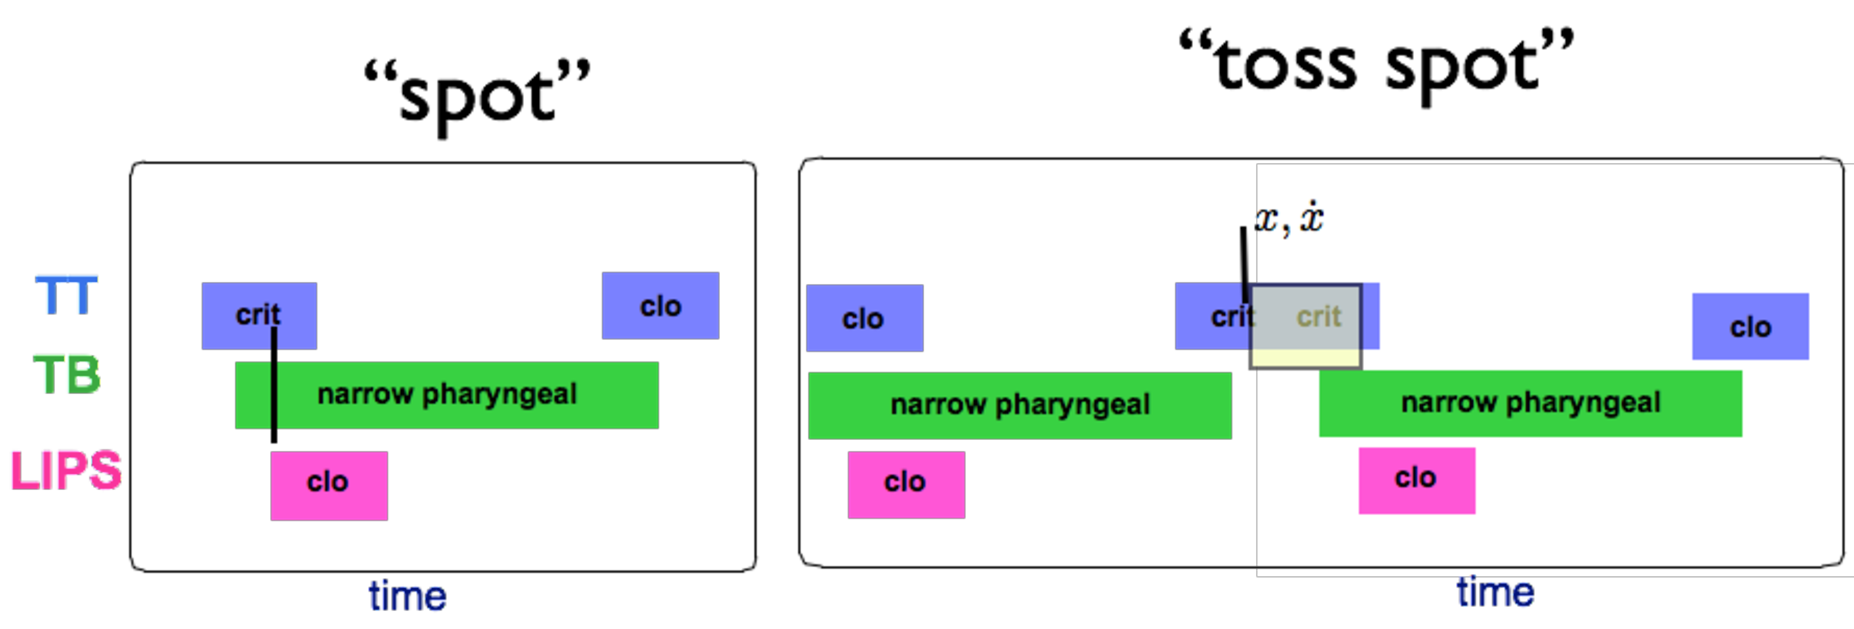
\includegraphics [width=\linewidth]{toss_spot}
\caption{Gestural scores. On the left for the word ``spot'' and on the right for the phrase ``toss spot.'' Rows represent (from the) top, gestures of the Tongue Tip, Tongue Body and Lips. See text. Shaded area represents interval of time during which state of tongue tip is not changing.}
\label{fig:spot}
\end{figure} 

\begin{figure}[htpb]
\center{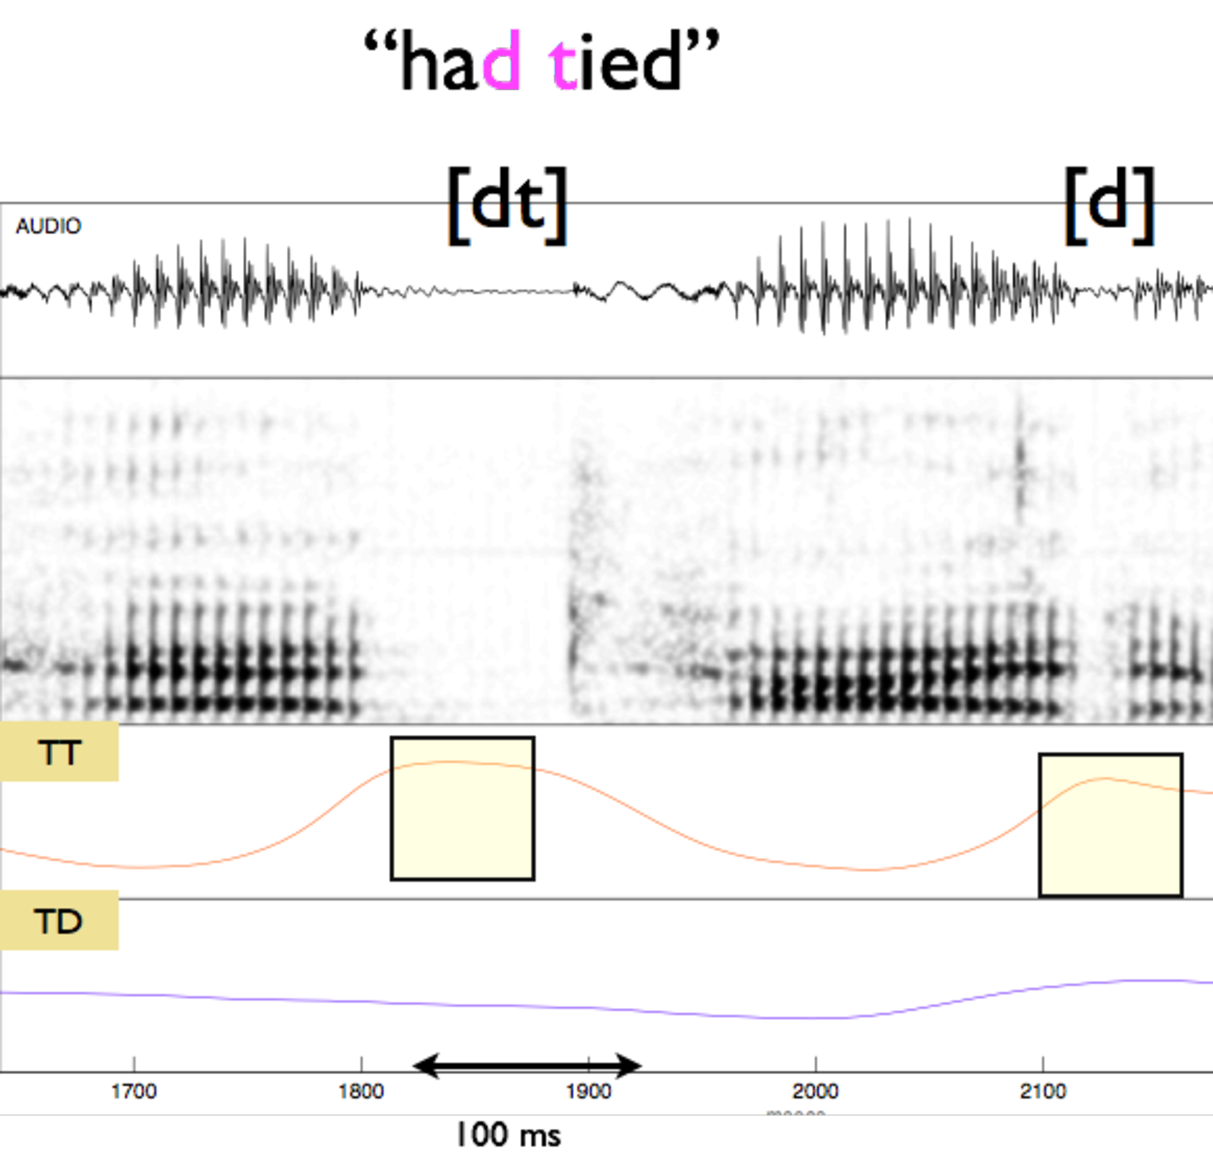
\includegraphics [width=3in]{had-tied}}
\caption{Time functions of the vertical position of the Tongue Tip (TT) and Tongue Dorsum (TD) in the phase ``had tied.'' See text.}\label{fig:had-tied}
\end{figure}

The coupled oscillator model of syllable structure \citep{Goldstein2006} proposes a specific alternative to gesture sequencing, in which the clock machinery is separate from the particular gestures that form the syllable. In this model, the gestures composing a syllable are triggered by a system of planning oscillators (clocks) that are coupled to one another in distinct modes. Each planning oscillator triggers activation of a gesture. Specifically, clocks that trigger gestures comprising onset consonants (consonants preceding the vowel in a syllable) are coupled in-phase (the most stable mode) to the vowel gesture and clocks that trigger gestures comprising coda consonants (consonants following the vowel in a syllable) are coupled in anti-phase mode to the vowel. If every gesture is triggered at phase 0 degrees of its planning oscillator, then two gestures that are coupled in phase will be triggered synchronously. This synchronous triggering explains data that show that the onset of articulatory movement for an onset consonant and for the following vowel begin at roughly the same time \citep{Goldstein2006}.  When two gestures are coupled in anti-phase mode, however, they will be triggered a half-period apart in time, which would be consistent with the observed time lag between the onset of the vowel gesture and the onset of a coda consonant gesture \citep{Goldstein2006}.   The ensemble of oscillators can be formally represented as a (coupling) graph, and Figure 3 shows the coupling graph for the word ``tab.'' Green edges represent in-phase coupling and the dashed red edge represents anti-phase coupling. Note that the same graph topology would underlie the timing of gestures in any CVC syllable, and in that sense, the clock is separate from, and independent of, the particular gestures that are deployed. The model has been used to explain patterns of syllable typology, acquisition \citep{Nam2009}, asymmetric coordination patterns in onset vs coda \citep{Marin2010}, and weight, and it has been used as a diagnostic for the syllable structure of complex pre-vocalic clusters \citep{Hermes2013, Shaw2009}. 


\begin{figure}[htpb]
\center{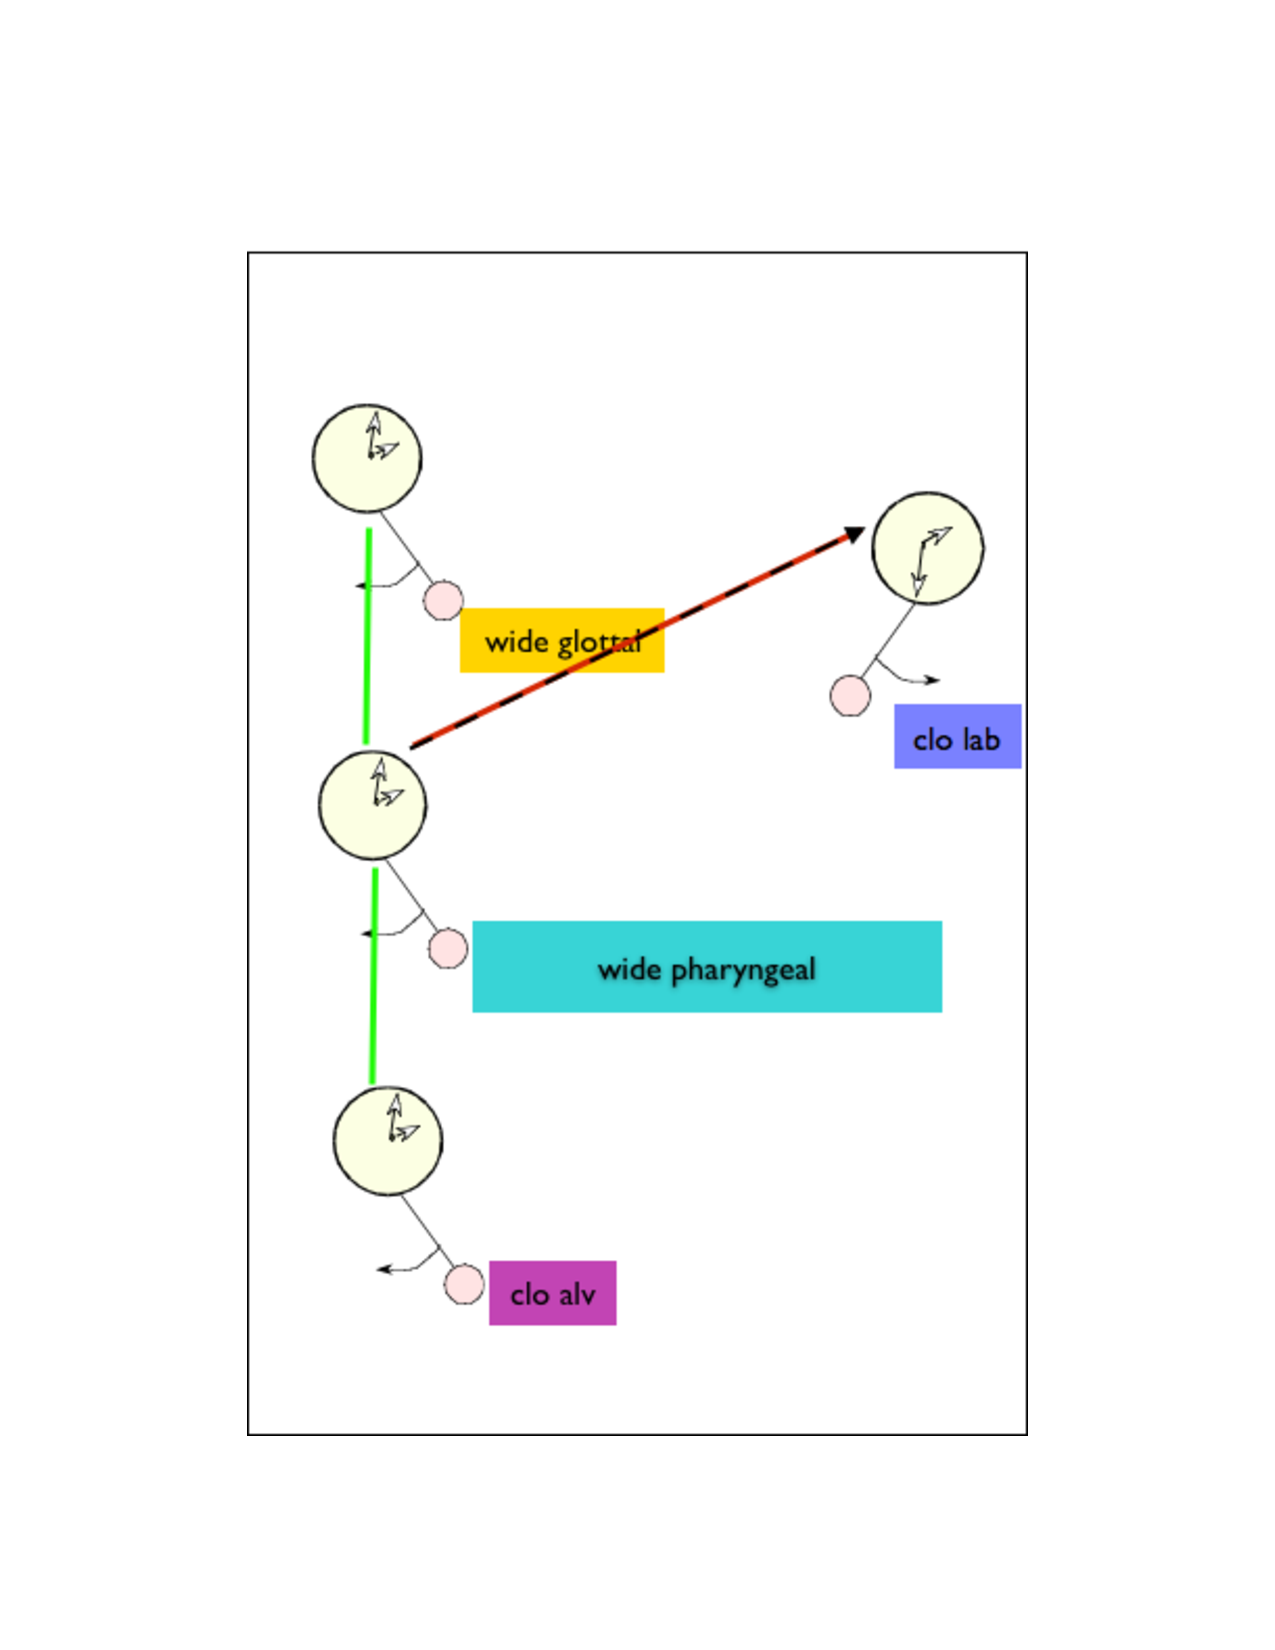
\includegraphics [height=5in]{clockworks2}}
\label{fig:clockworks}
\caption{Coupling graph for the word ``tab.'' Each clock represents one of the gestures in the word and they are the nodes of the coupling graph.  From the top down the left, these are glottal abduction for the initial /t/,  pharyngeal constriction (for the vowel), and tongue tip closure for the /t/. At the right is the lip closure for /b/.   Green lines are graph edges that represent in-phase coupling and the red dashed line with arrowhead is the edge that represents anti-phase coupling. Boxes represent the gestural score for the the word (gesture activation over time) that results from running the coupled oscillator model.}
\end{figure}

The frequencies of the planning oscillator clocks are all defined with reference to the ticks of  an overall speech rate clock. Prosodically-induced lengthening can thus be modeled as slowing of the rate of this overall clock, as has been proposed in the $\pi$-gesture model \citep{Byrd2003}. Phrase edges are associated with local $\pi$-gestures, which function to slow the movements of all gestures that fall under the scope of the $\pi$-gesture. This model has been shown to account for the acoustic and kinematic correlates of boundary lengthening in a variety of languages (e.g. Greek; \citealt{Katsika2014}).

\subsection{Clocks in birdsong?}

Work on birdsong over the last 15 years has also revealed, within limits, separate control of timing and vocal organ activation patterns. Two areas of the avian cortex have been identified as significant  for the production of the song: HVC, a pre-motor nucleus, and RA (robust nucleus of the arcopallium).  HVC projects to RA, which in turn projects to the vocal motor neurons (and to midbrain vocal control areas). HVC was suspected to be a major site of timing control, and this was tested in a seminal study by Long and Fee \citeyearpar{Long2008}. Reasoning that cooling a brain region would result in a slowing of neural patterns, they used a miniature Peltier device to locally cool either HVC or RA. They found that cooling HVC resulted in slowing of the song, with the amount of slowing being proportional to the degree of cooling.  Further, the slowing was fairly linear throughout the song. Syllable durations, onset lags, gap durations between motifs were all slowed to roughly the same degree, indicating that something like an overall clock (like the proposed speech clock) was being slowed. Consistent with the independence of timing account, there was very little change at all in the actual acoustics of the song, indicating that the control of the activation patterns at the level of the motor neurons remained intact, just spread out in time. (In other words, the rate at which the motor commands were issued was slowed down, but the commands were not changed, so the frequencies of the song were not altered by slowing). Conversely, even though spiking was decreased by cooling RA, the ability of (uncooled) HVC to drive RA and produce typical song speeds was not impaired, thus providing evidence for localizing timing control in HVC.

A more recent study of cooling from a different lab using canaries \citep{Goldin2013} found that with more extreme cooling of HVC, the song begins to break down, exhibiting period-doubling of respiratory patterns, causing the emergence of additional syllables. The authors provide a formal model that predicts these transitions from the nonlinear interaction between the (hypothesized) neural pulse train (from HVC) and the dynamics of the respiratory cycle. Interestingly, this kind of period-doubling can also be observed in ``gestural intrusions'' human speakers produce when repeating phrases like ``top cop", and a similar dynamical account has been proposed, less formally \citep{Goldstein2007}.  That study found that when speakers produce such phrases repeatedly, they will begin to produce an ``extra'' copy of the tongue tip gesture of /t/ concurrently with the
initial tongue dorsum gesture of ``cop'' (resulting in a co-produced /k͡t/) and conversely an extra tongue dorsum gesture during the initial tongue tip gesture of ``top''. These extra cycles of repeated tongue tip or tongue dorsum movement can be analyzed as a period doubling -- 2:1 to 1:1 transitions in frequency mode locking between the tongue tip (or tongue dorsum) oscillators and the lip oscillator of the syllable-final lip gesture (there is a lip gesture in every syllable, but a tongue tip or dorsum gesture only every other syllable; \citealt{Goldstein2007}).
Since such period-doubling transitions in birdsong are analyzed by \citet{Goldin2013}  as resulting from a presumed slowing of a clocking pulse in HVC, the results do not contradict the main finding and conclusion of the earlier work of Long and Fee. However, there is disagreement between the two research groups as to the nature of the temporal code in HVC and how it interacts (or not) with the rest of the system, as will be fleshed out a bit in the last section.

\subsection{Brain-cooling in speech}

The technique of focal brain cooling was recently employed with humans for the first time \citep{Picardo2016} with patients undergoing brain surgery for either epilepsy or tumor resection. Cooling was applied in up to 4 locations in each subject, two in Broca's area within the left inferior frontal gyrus (IFG) and the others in the precentral gyrus (speech motor cortex). The hypothesis was that there would be a double dissociation with cooling in Broca's area causing changes in speech timing but not in articulatory quality, and that cooling the speech motor cortex would disrupt articulation, but not timing. Patients were recorded producing the digits from 1 to 20 or the names of the days of the week (one sequence per trial, with breaks between trials) while respective sites were being cooled, and also during control trials with no cooling. The utterances were judged for quality via crowd-sourcing on a scale from 0 (extremely degraded) to 1 (typical/normal). Timing was determined through durational measurements. Results supported the double dissociation. Cooling Broca's area resulted in changes to speech timing. Typically utterances  were slowed down (both the actual articulation of words and the gaps between them were stretched), but some cases speeding up occurred. No effect was found on judged quality. When the speech motor cortex was cooled, ratings shifted to more degraded, with no effect on timing.

To examine the slowing more carefully, the authors generously made available the data from two of their subjects, one of which is analyzed here.  Figure 4(a-b) shows boxplots for durations of the names of the days of the week (excluding pauses between names); on the left, control utterances are displayed and on the right, the trials with cooling of Broca's area. Results show fairly uniform slowing across the names of the days of week, except for ``Friday,'' which shows less slowing. Somewhat surprising is that Friday is the shortest of all the words (even in the controls); there is certainly no tendency for list-final prosodic lengthening here. In terms of intonation, M-W generally appear to be produced with an extended High tone. Falling begins on ``Thursday'' and ``Friday'' is generally produced on a Low tone. So it is possible that the durations follow the prominence profile of the utterance. By itself, however, this does not explain the reduced percentage of slowing on ``Friday.'' Another possibility is that cooling in Broca's area has a bigger effect on more complex syllable types (for example with coda consonants or clusters). The initial syllables of the days of the week all have closed syllables (with coda consonants) except ``Friday''. To test this, the durations of the initial syllables and final syllable (``day'') were analyzed separately, and the magnitude of lengthening of initial (dark blue bars) vs. final (light yellow bars) syllables are shown in Figure 5. Magnitude of lengthening is calculated as the ratio of the median duration of that syllable when cooled divided by the median duration of controls. The lengthening of the (open) syllable ``day'' is approximately the same across all the days' names. The lengthening of the first syllable in ``Friday'' (an open syllable) is about the same as for ``day'', while the other first syllables (that are closed) lengthen more. The most lengthening is observed on the first syllable of ``Wednesday'', which is also the most complex syllable, closed with a coda cluster.  This is consistent with the hypothesis that more complex syllables exhibit more slowing 
due to cooling in Broca's area.

\begin{figure}[htpb]
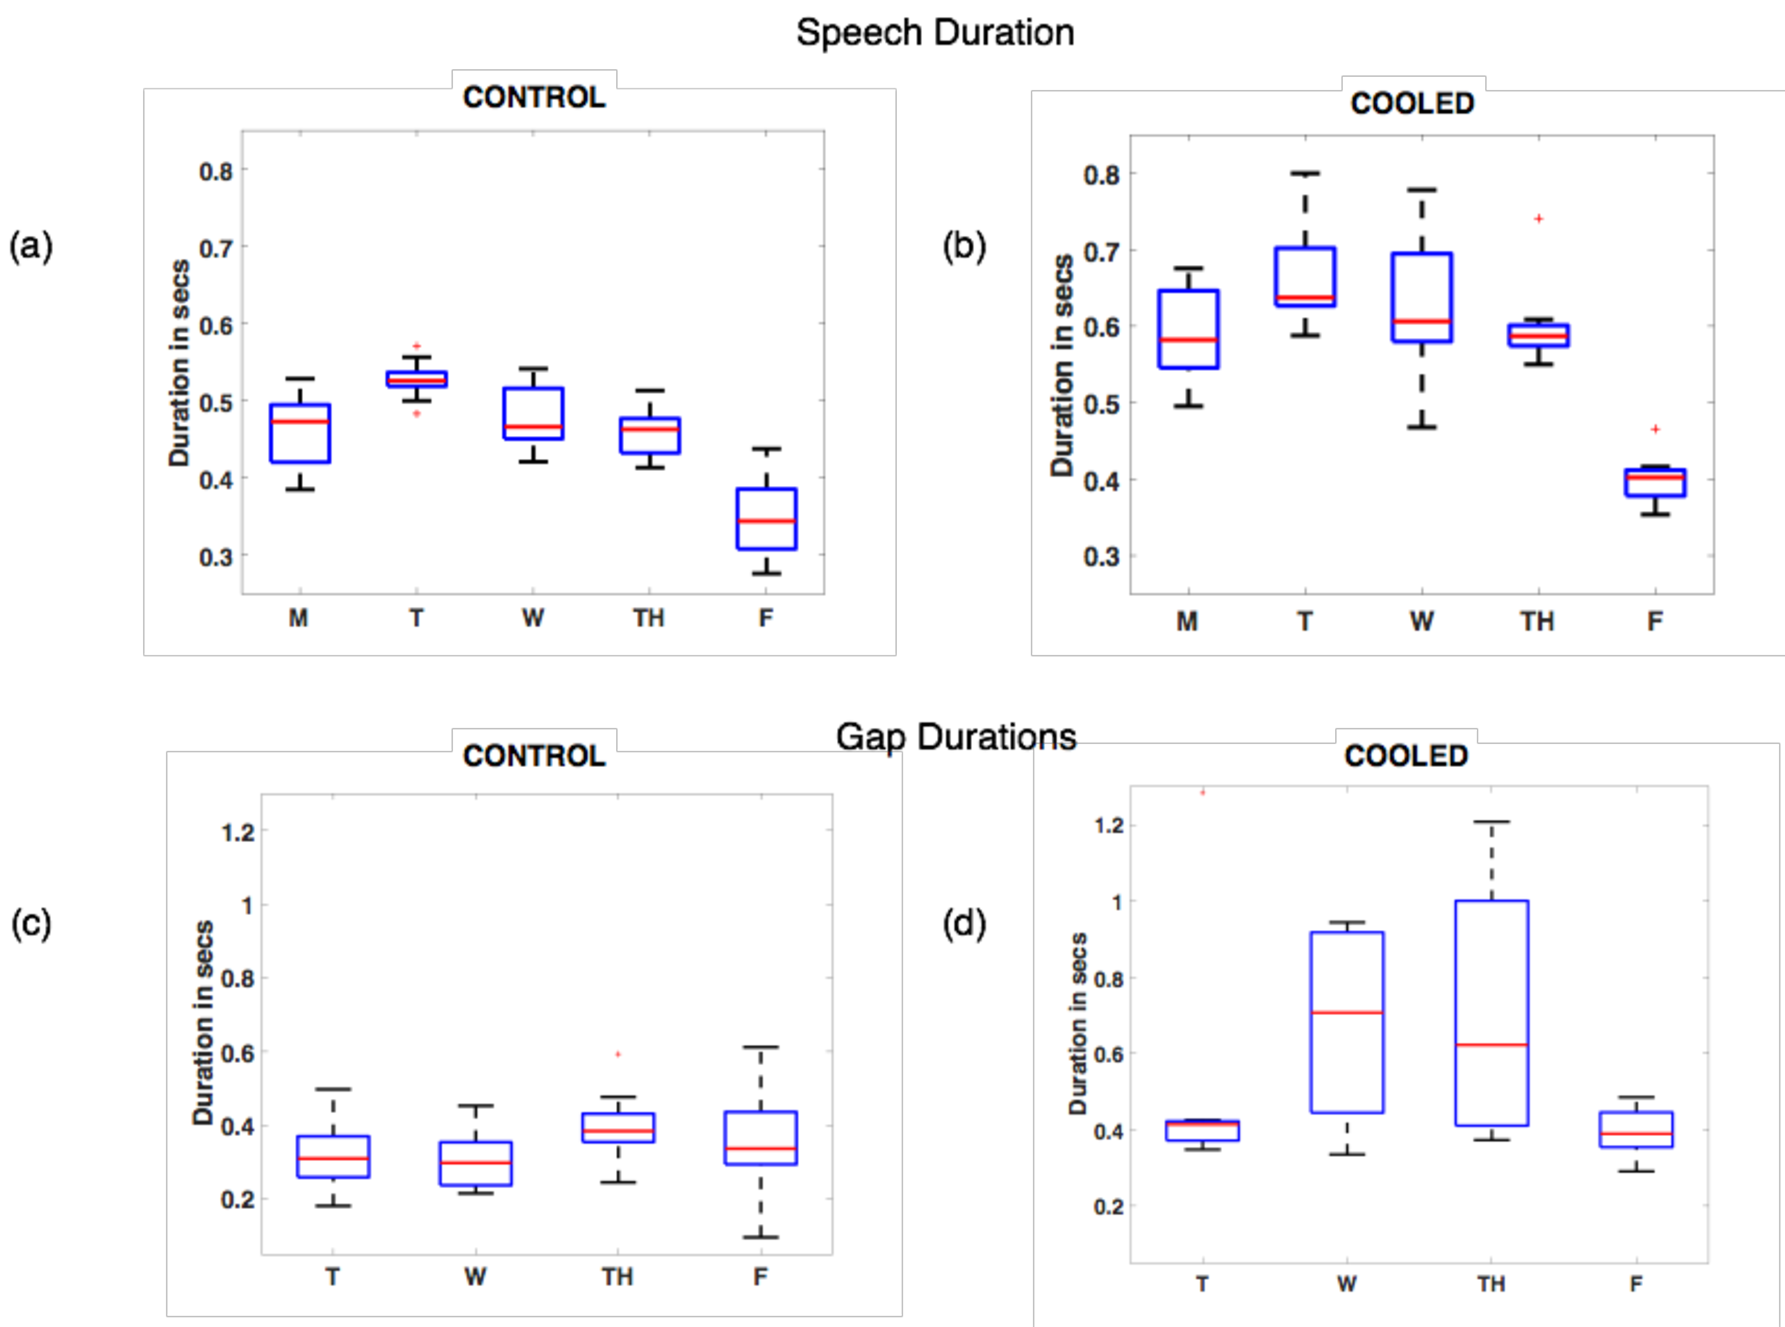
\includegraphics [width=\linewidth]{durations}
\label{fig:durations}
\caption{(a-b) Boxplots of duration of the names of days of the week from one patient. Control condition is shown in (a), cooling Broca's area is shown in (b).   (c-d) Boxplots of silent gap durations before the production of the names of the week Tuesday-Friday.  Control condition is shown in (c), cooling Broca's area is shown in (d). }
\end{figure}

Figure 4(c-d) shows the durations of the silent period before initiation of the words ``Tuesday'' to ``Friday'' from the time of completion of the preceding word. This shows a strikingly different pattern from that exhibited by the word durations. The silent gaps before ``Tuesday'' and ``Friday'' show very little effect, while the gaps before ``Wednesday'' and ``Thursday'' show almost 3:1 lengthening. The pattern is reminiscent of the classic pattern of recall in short-term memory \citep{Deese1957, Ebb, BrownNeath}. The items in the middle of the list have more competitors on either side and therefore more interference, although many other models have been proposed. Such results could be modeled by a competitive queuing model of sequence selection \citep{Bullock2002}, depending on exactly how the parameters are set. In any case, it is clear that more is going on than just clock slowing when Broca's area is cooled, unlike what is observed in zebra finch, though clock slowing is also going on.

\begin{figure}
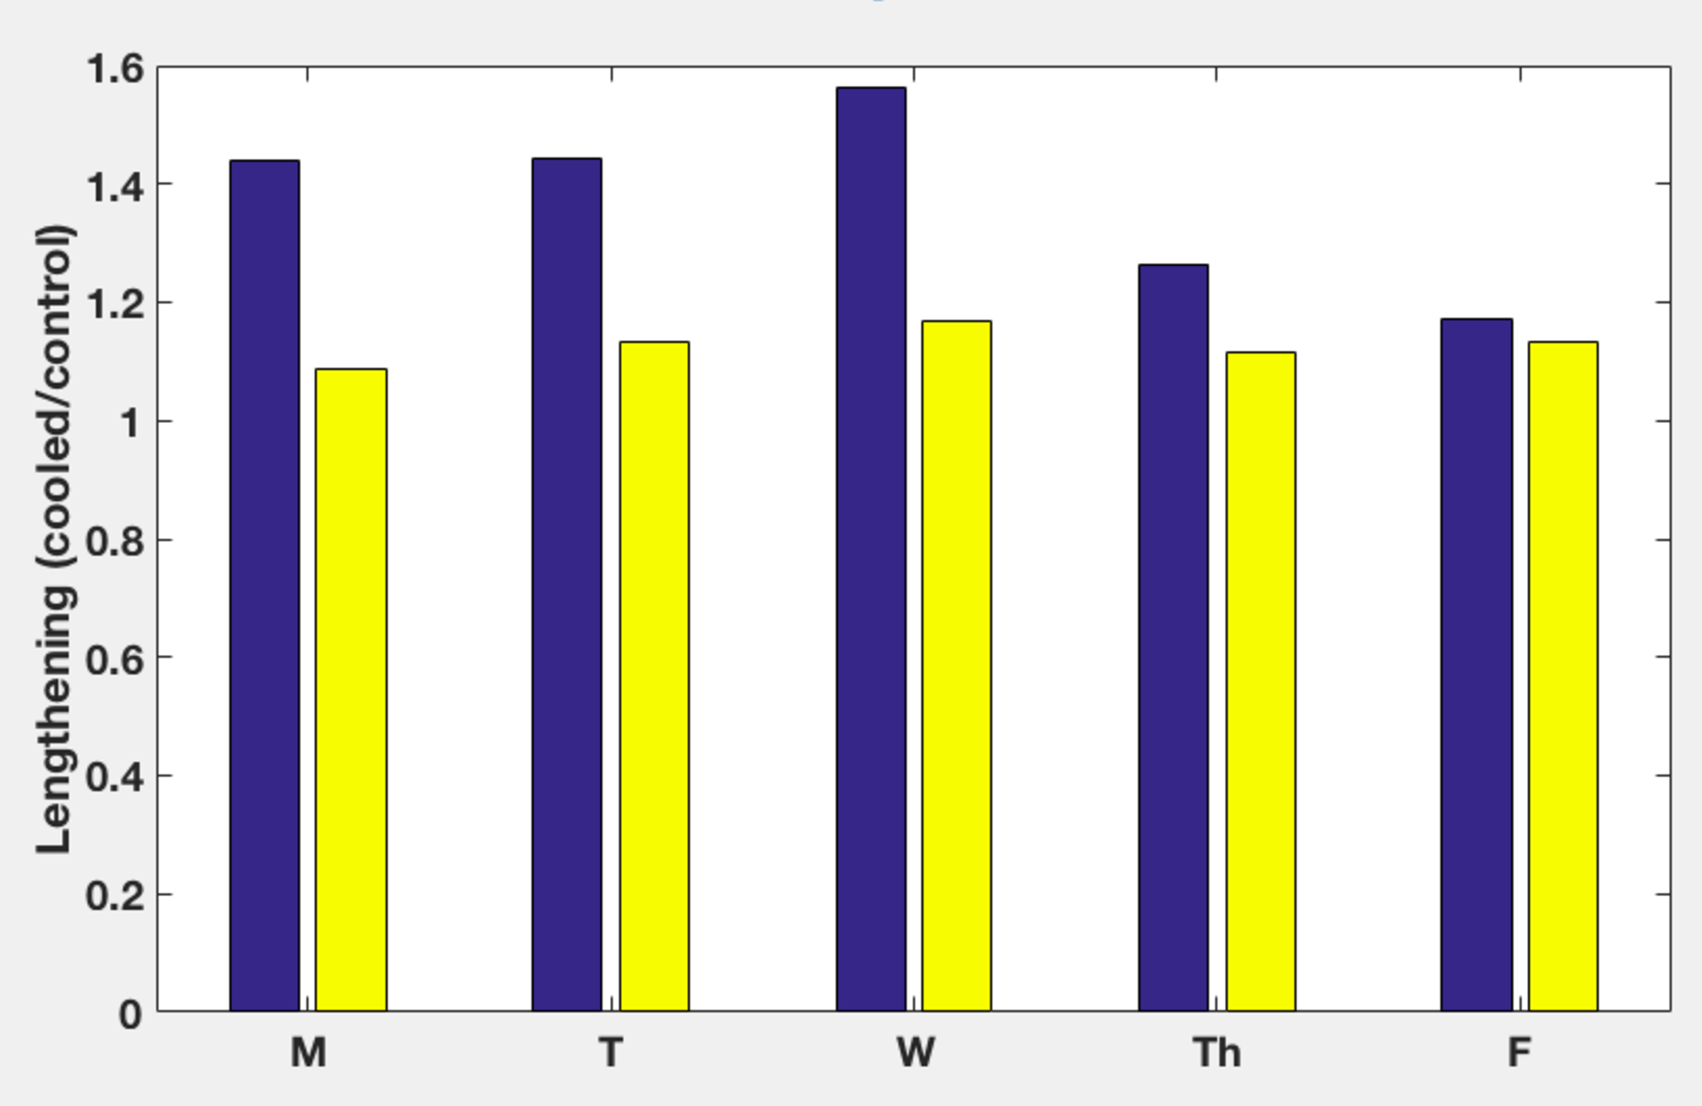
\includegraphics [width=5in]{lengthening}
\caption{Magnitude of lengthening of initial (dark blue bars) vs. final (light yellow bars) syllables of the names of the days of the week. Magnitude of lengthening is calculated as the ratio of the median duration of that syllable when cooled divided by the median duration of that syllable in the uncooled control condition.}
\end{figure}

In summary, the results with humans generally confirm the dissociation of the timing clock from the articulatory gestural patterning that it paces.  Differently from birds, however, where gaps between syllables and motifs were slowed in a roughly similar way to the actual song syllables, the gaps between the days of the week showed marked differences in response to cooling, depending on position in the list (for the one patient examined). This suggests that even for an over-learned list, mechanisms of selection of discrete individual words must still be in play, while for the bird, the entire song may just ``run off'' at different rates. This may be related to the relative lack of flexibility in the zebra finch song. Also the possible effect of syllable complexity on the magnitude of slowing also suggests that more is going on for humans when Broca's area is cooled than just uniform slowing of the clock.
 
\subsection{Continuous vs discrete temporal representations}
The last point brings up the nature of temporal coding that characterizes the representation in HVC of the bird (compared for example to the clock model proposed for speech discussed above). The work of Fee and collaborators has consistently supported the view that the representation is a continuous-time representation of the song (in 10 ms or so slices). This is based on the earlier discovery  \citep{Hahnloser2002}
of individual cells that burst sparsely in the song at a fixed lag from song onset. Theoretically then, there could be such cells for each 10ms sample in the sound, and they jointly produce a continuous representation. Further, their hypothesis is that the continuous-time representation completely drives (or enslaves) the downstream activity in RA and the vocal muscles to reproduce the song \citep{Long2008}, which is why the slowing does not result in distortions to the song (but cf. the results discussed earlier with extreme values of cooling). An alternative discrete view was proposed by the Margoliash and Mindlin group \citep{Amador2013}. After discovering that it was possible to decompose the dynamical parameters governing song production into discrete gestures, as discussed above, they found that burst times of HVC neurons projecting to RA tended to be synchronized with the gestural extrema, for 14 of the 15 sites they examined with recordings of single neurons. This is exactly what would be predicted by coupled oscillator model of syllable structure described above: the clock mechanism generates a sequence of bursts that trigger their corresponding gestures. However, attempts to replicate this finding with a substantially larger population of cells, in both Long's lab \citep{Picardo2016} and Fee's \citep{Lynch2016}, failed to replicate this finding. It is unclear why this is, apart from possible differences in sites examined and the types of electrodes used. It would not be surprising to find that both continuous and discrete representations co-exist in different subpopulations of neurons. The discrete representation would be useful during learning to produce individual ``pieces'' of the song on the way to mastery (assuming a continuous representation of the target song in auditory areas is any case available to the system). Consistent with this, \cite{Lynch2016} did find evidence of 10-Hz rhythmicity locked to song syllables, which was significant for HVC projections to Area-X (basal ganglia loop employed in learning) but not for HVC projections to RA. Given the stereotypy of zebra finch song, it is not surprising that a continuous-time representation could work. Obviously in the case of speech, we are capable of producing novel forms, and for that a discrete representation like the coupled oscillator model is really the only viable candidate (or compatibly,  models like that of Bohland and Guenther, e.g., \citet{Bohland2010}).


\section{Summary}
%\label{sec:summary}

Speech and birdsong share the property that their production can be decomposed into a sequence of discrete motor actions. In addition, the control of those actions is governed by a  separate timing representation.  The nature of the timing representation appears to be substantially different however, possibly due to the essential combinatoriality and productivity of human speech, though there is a lot still unknown about both speech and birdsong in this regard. It is interesting to consider why they should be as similar they are. One functional similarity is that while they are both species-specific capabilities, in both cases the specific behavioral forms must be learned by individuals (in the bird species in which the song is learned from experience). There are other odd similarities as well, such as the compatible frequency of their syllable rates. This flies in the face of hypotheses that the duration of the syllables in speech is related to the natural frequency of the jaw (e.g., \citealt{Davis}). A more likely cause may be the similarity of their auditory systems. In any case, the existence of a model system that can be probed in ways that speech cannot provides the opportunity of deepening our understanding of speech, particularly when we observe the particular places in which the systems diverge.



%\section*{Abbreviations}
\section*{Acknowledgements}
Many thanks to Michael Long and Kalman  Katlowitz for making their data available, and to Jelena Krivokapic, Mairym Llorens, Sarah Bottjer, and two anonymous reviewers for their comments on an earlier draft.



\printbibliography[heading=subbibliography,notkeyword=this]



\end{document}

